% !TEX root = ../my-thesis.tex
%
\chapter{Results}
\label{sec:results}

As discussed in \ref{sec:overfit}, the model architecture should be neither too simple to be underfitted and nor too complex to be overfitted. 
In this case, the dataset and the relationship between the dependent variables and the independent variable were pretty straightforward for the models to predict the essence of lifts. 
The dataset that is relevant to the problem being solved ensures that the model learns meaningful patterns and relationships, enhancing accuracy
\cite{gudivada2017data}.

Note that the dataset has high precision and accurate values and the fact that the minimal presence of null values further contributed to desirable output. With that being said, even though cross validation has been used to prohibit any sort of overfitting, the results were still satisfying.
It is imperative to divide data into training, validation, and testing sets to fairly evaluate the model's accuracy on unseen data. Moreover, note that a larger dataset is preferred as it allows the model to learn diverse patterns and reduces the risk of overfitting, ultimately leading to better accuracy.





\section{Confusion Matrix}




The confusion matrix is a table that is often used to describe the performance of a classification model on a set of data for which the true values are known. In this case, the matrix is a 2x2 matrix representing two classes (0 and 1). Each cell in the matrix represents a count of instances where the predicted class corresponds to the row and the actual class corresponds to the column.


\begin{figure}[htb]
	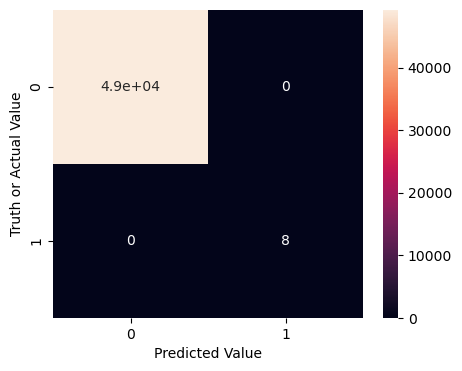
\includegraphics[width=\textwidth]{resources/confusion.png}
	\caption{The loaded DataFrame}
	\label{fig:confusion}
\end{figure}


According to Fig. \ref{fig:confusion}, the top-left cell (49271) indicates that the model correctly predicted 49271 instances of class 0 as class 0.
The bottom-right cell (8) indicates that the model correctly predicted 8 instances of class 1 as class 1.
The other two cells (top-right and bottom-left) are both 0, which means that the model made no errors in classifying instances from one class into the other.
Classification Report:
This report provides a summary of various metrics used to evaluate the model's performance.

Precision: Precision is the ratio of correctly predicted positive observations to the total predicted positives. In both classes 0 and 1, the precision is 1.00, which means that all instances predicted as positive (class 1) were actually correct.

Recall: Recall (also known as Sensitivity or True Positive Rate) is the ratio of correctly predicted positive observations to the all observations in the actual class. Again, for both classes, the recall is 1.00, indicating that the model correctly identified all positive instances.

F1-score: The F1-score is the weighted average of precision and recall. It considers both false positives and false negatives. Since both precision and recall are 1.00, the F1-score is also 1.00 for both classes.

Support: The number of actual occurrences of each class in the test dataset. In this case, there are 49271 instances of class 0 and 8 instances of class 1.

Accuracy: Accuracy is the ratio of correctly predicted observations to the total observations. Here, the accuracy is 1.00, which means the model predicted all instances correctly.

Macro Average: The macro average calculates the metric independently for each class and then takes the average. In this case, since precision, recall, and F1-score are 1.00 for both classes, the macro average is also 1.00.

Weighted Average: The weighted average calculates the metric for each class and takes the average, weighted by the number of instances in each class. Since all metrics are 1.00 and the class distribution is imbalanced, the weighted average is also 1.00.

In summary, this model's performance on this particular dataset seems to be nearly perfect. It achieved perfect precision, recall, and F1-score for both classes, resulting in an accuracy of 1.00. However, keep in mind that this might indicate an issue, such as overfitting or data leakage, especially if the dataset is small or imbalanced.

* put confusion\_matrix figure




\section{Section 2}
\label{sec:results:sec3}



\section{Conclusion}
\label{sec:results:conclusion}




\section{Future Work}
\label{sec:results:future}

a chatbot to chat with csv can be used to talk to the datasets.